\documentclass[english,master]{liumaiex}
% Options are english, swedish, bachelor and master


%=========================================================================%
%
% Add optional packages. Some are almost essential. 
%
%=========================================================================%
\usepackage{amssymb}
\usepackage{amsmath}
\usepackage[dvips]{graphicx}
\usepackage{xcolor}
\usepackage{amsthm}
\usepackage{comment}
\usepackage{parskip}
\usepackage{tikz}
\usepackage{lipsum}
\usepackage{makecell}
\usepackage{pgfplots}
\pgfplotsset{compat=1.18}

\theoremstyle{plain}
\newtheorem{proposition}{Proposition}[section]
\newtheorem{corollary}[proposition]{Corollary}
\newtheorem{lemma}[proposition]{Lemma}
\newtheorem{theorem}[proposition]{Theorem}
\newtheorem{conjecture}[proposition]{Conjecture}
\theoremstyle{definition}
\newtheorem{definition}[proposition]{Definition}
\newtheorem{example}[proposition]{Example}
\newtheorem{remark}[proposition]{Remark}

\newcommand\todo[1]{\textcolor{red}{#1}}
\newcommand{\sgn}{\text{sgn}}
\newcommand{\tr}{\text{tr}}

\begin{document}


%=========================================================================%
%
% Information to fill-in
%
%=========================================================================%
\title{The title of the thesis}
\author{Erik Jonasson}
\shortauthor{Jonasson}
% If there are several authors, just enter the names separated by comma or 'and'
\publishmonth{June}
\publishyear{2024}
%\city{City} % Has Linköping as default
%\department{Department name} % Has MAI as default
\supervisor*{Hans Lundmark}
% To add another supervisor, just use the command again
\examiner*{Fredrik Andersson} % use a star to add department automatically
% \supervisor also accepts the star format
%\level{G2} % Not needed when bachelor/master is set in options
%\credits{16 hp} % Not needed when bachelor/master is set in options
\regnumber{The number your thesis gets from administrators}
\enkeywords{Keyword 1, keyword 2, etc.}
\svkeywords{Nyckelord 1, nyckelord 2, etc.}
\publishurl{The url to the thesis}
%\pdfauthor{Name} % Needed if name is complex
%\pdftitle{Title} % Needed if title is complex
%\pdfkeywords{Keywords} % Needed if keywords are complex
%\pdfsubject{Subject} % Optional

\maketitle


%=========================================================================%
%
% Introductory part: Abstract, Acknowledgements, etc 
%
%=========================================================================%
\pagenumbering{roman}
\section*{Abstract}

A summary of the thesis, presenting the important results.

\placeenkeywords
\placeenurl

\newpage

% \cleardoublepage
% \begin{otherlanguage*}{swedish}
% \chapter*{Sammanfattning}

% You can write a swedish abstract in this environment to get
% correct (swedish) formatting and hyphenation

% \placesvkeywords
% \placesvurl
% \end{otherlanguage*}

% \chapter*{Acknowledgements}

% Acknowledgements and thanks to people that have helped you.

% \chapter*{Nomenclature}

% The notation you will use in the thesis

\tableofcontents
%\listoffigures
%\listoftables

\newpage



%=========================================================================%
%
% Main part of the thesis
%
%=========================================================================%
\pagenumbering{arabic}

\section{Introduction}

The objective of this thesis is to study the high-frequency limit of the Novikov equation. Taking the high-frequency limit of the Novikov equation yields the following equation
\begin{equation} \label{eq:Novikov_high_freq}
	m_t + ((um)_x + 2u_xm) u = 0,\quad m = u_{xx},
\end{equation}
where $u = u(x, t)$. The Novikov equation is a member of the family of peakon equations. The study of high-frequency limits of peakon equations have been done for the Camassa--Holm (CH) equation and the Degasperis--Procesi (DP) equation.

These are integrable systems, which are non-linear differential equations where the solutions can be reduced to a finite number of algebraic operations and integrations. Such systems are rare, as most non-linear differential equations lack explicit solutions.

\subsection{Peakon background}

In 1834 John Scott Russell discovered a solitary wave in a canal. The wave was created by a boat traveling along the canal. The wave was solitary in that it maintained its shape and speed as it traveled along the canal.

Diederik Johannes Korteweg and Gustav de Vries continued the study of solitary waves and they were the first to derive a partial differential equation (PDE) that describes solitary waves. In 1895 they discovered the now famous Korteweg--de Vries (KdV) equation
\begin{equation}
	u_t + u_{xxx} - 6uu_x = 0,
\end{equation}
that describes solitary waves in shallow water.

It was not until much later in 1965 that Zabusky and Kruskal \cite{Zabusky1965} discovered numerically that the KdV equation has solutions of solitary travelling waves that can interact with each other without changing shape. They called these solitary waves solitons. Solitons have since been studied in many fields such as fluid dynamics, optics, and quantum mechanics.

In 1993\cite{Camassa_1993}, while working on an integrable model of one-dimensional dispersive waves in shallow water Camassa and Holm discovered the first PDE which admit peakon (peaked soliton) solutions. The Camassa--Holm (CH) equation
\begin{equation} \label{eq:CH}
	m_t + (um)_x + u_xm = 0,\quad m = u - u_{xx},
\end{equation}
opened up the door for many other PDEs with peakon solutions. The peakon traveling wave moves at a speed based on its maximum height, at which
it has a sharp peak (jump in derivative). These peakon solutions have are one the following form
\begin{equation} \label{eq:peakon}
	u(x, t) = \sum_{k = 1}^{N} m_k(t) e^{-|x - x_k(t)|}.
\end{equation}
Later the Degasperis--Procesi equation
\begin{equation} \label{eq:DP}
	m_t + (um)_x + 2u_xm = 0,\quad m = u - u_{xx}.
\end{equation}
was studied by Degasperis and Procesi in 1999 \cite{Degasperis_1999}. Both the CH and DP equations share similar properties with the Novikov equation. For a more detailed discussion of the peakon equations and their properties, see the comprehensive overview by Lundmark and Szmigielski \cite{Lundmark_2022}.

This brings us back to the Novikov equation
\begin{equation} \label{eq:Novikov_high_freq}
	m_t + ((um)_x + 2u_xm) u = 0,\quad m = u - u_{xx}.
\end{equation}
It was discovered by Vladimir Novikov in a classification of cubically nonlinear PDEs admitting infinitely many symmetries \cite{Novikov_2009}, with Hone and Wang \cite{Hone2008} later providing a Lax pair for it.

\subsection{High-frequency limit}

As mentioned at the start the focus of the thesis is on the high-frequency limit of the Novikov equation. The high-frequency limit is obtained by substitution of $x \mapsto \epsilon x$, $t \mapsto \epsilon t$, $m \mapsto -\epsilon^{-2} m$, and letting $\epsilon \rightarrow 0$. This limit gives the high-frequency Novikov equation \eqref{eq:Novikov_high_freq}.

Both the CH and DP equations have been studied in the high-frequency limit.  The high frequency limit of the Camassa--Holm equation yields the Hunter--Saxton equation \cite{HunterSaxton_1991,HunterZheng1994} for nematic liquid crystals. The high frequency limit of the Degasperis--Procesi equation yields the derivative Burgers equation \cite{Kohlenberg_2007, Lundmark_2008}.  The only difference between all three of the original equations and their respective high-frequency limit is that $m = u_{xx}$ instead of $m = u - u_{xx}$.
\begin{center}
  \begin{tabular}{l|c|c}
    & $m=u-u_{xx}$ & $m=u_{xx}$ \\
    \hline
    $m_t + (um)_x + u_xm = 0$ 
	& \multicolumn{1}{l|}{Camassa--Holm} & \multicolumn{1}{l}{Hunter--Saxton} \\
    \hline
    $m_t + (um)_x + 2u_xm = 0$ 
	& \multicolumn{1}{l|}{Degasperis--Procesi} & \multicolumn{1}{l}{Derivative Burgers} \\
    \hline
    $m_t + ((um)_x + 2u_xm)u = 0$ 
	& \multicolumn{1}{l|}{Novikov} & \multicolumn{1}{l}{HF Novikov} \\
  \end{tabular}
\end{center}

All three high-frequency limits also admits piecewise linear solutions on the following form
\begin{equation} \label{eq:linear_peakon}
	u(x, t) = \sum_{k = 1}^{N} m_k(t) |x - x_k(t)|.
\end{equation}
For the HF Novikov equation the time derivative of $x_k$ and $m_k$ will be governed by the following ODEs
\begin{equation} \label{eq:peakon_odes}
\dot{x}_k = u(x_k)^2, \quad
\dot{m}_k = -m_ku_x(x_k)u(x_k).
\end{equation}
Dots denote $\frac{d}{dt}$ as usual. $u(x_k)$ and $u(x = x_k,t)$ is given by
\begin{align}
	u(x_k) &= \sum_{i = 1}^{N} m_i(t) |x_k - x_i(t)|, \\
	u_x(x_k) &= \sum_{i = 1}^{N} m_i(t) \sgn(x_k - x_i).
\end{align}
The $u_x$ isn't defined at $x = x_i$ but we define it to be the average of the left and right limits and we will see that this is consistent with the PDE.  See Appendix(\ref{sec:DerivationODE}) for the proof that the HF Novikov equation admits piecewise linear solutions on the form of equation \eqref{eq:linear_peakon} and that the ODE-system is compatible with the PDE.

The peakon equations and their respective high-frequency limits share many similarities. The ODEs for both equations share the same form, but the $u(x_k)$ and $u_x(x_k)$ are different. Both the regular and HF Novikov equations only have $x_i$'s that travel to the right due to the $u(x_k)^2$ term in the ODEs.
\begin{center}
  \begin{tabular}{l|c|c}
    & $u=\sum_{i=1}^n m_i e^{-|x-x_i|}$ & $u=\sum_{i=1}^n m_i |x-x_i|$ \\[3pt]
    \hline
    \makecell[l]{
	$\begin{aligned}
		\dot{x}_i &= u(x_k),\\
		\dot{m}_i &= -\phantom{2}m_i u_x(m_i)
	\end{aligned}$}
	& \multicolumn{1}{l|}{Camassa--Holm} & \multicolumn{1}{l}{Hunter--Saxton} \\
    \hline
    \makecell[l]{
	$\begin{aligned}
		\dot{x}_i &= u(x_k),\\
		\dot{m}_i &= -2m_i u_x(m_i)
	\end{aligned}$}
	& \multicolumn{1}{l|}{Degasperis--Procesi} & \multicolumn{1}{l}{Derivative Burgers} \\
    \hline
    \makecell[l]{
	$\begin{aligned}
		\dot{x}_i &= u(x_k)^2,\\
		\dot{m}_i &= -\phantom{2}m_i u_x(m_i) u(x_i)
	\end{aligned}$}
	& \multicolumn{1}{l|}{Novikov} & \multicolumn{1}{l}{HF Novikov} \\
  \end{tabular}
\end{center}


\section{Preliminaries}

\subsection{Lax pairs}

Lax pairs are a mathematical framework used to analyze and solve certain types of integrable systems. They are the main tool used to solve peakon equations. The concept of Lax pairs was introduced by Peter Lax in 1968 \cite{Lax_1968}. A Lax pair consists of two operators, $L$ and $A$, that satisfy a specific compatibility condition. The existence of a Lax pair for a nonlinear PDE is a strong indicator of the equation's integrability. It allows the application of powerful analytical methods to find exact solutions and conservation laws. In many cases, Lax pairs are represented in matrix form, enabling a more straightforward application of the IST method.

\subsubsection*{Zero curvature representation}

The zero curvature representation is a generalization of the Lax pair, consisting of a pair of linear equations
\begin{equation}
	\partial_x \psi = U \psi, \quad \partial_t \psi = V \psi,
\end{equation}
that satisfy the zero curvature condition
\begin{equation}
	\partial_t U - \partial_x V + [U, V] = 0.
\end{equation}
The condition comes from equating the mixed partials $\partial_t \partial_x \psi = \partial_x \partial_t \psi$. The matrices $U$ and $V$ are called the Lax pair. The zero curvature condition is only satisfied if the Lax pair is integrable. 
\begin{example}
The KdV has the following Lax pair
\begin{subequations}
  \begin{equation}
    \partial x \psi =
    \begin{pmatrix}
      0 & 1 \\
      u - \lambda & 0
    \end{pmatrix}
	\psi,
  \end{equation}
  \begin{equation}
    \partial t \psi =
    \begin{pmatrix}
      -u_x & 2u + 4\lambda \\
      2u^2 - u_{xx} + 2u\lambda - 4\lambda^2 & u_x
    \end{pmatrix}
    \psi.
  \end{equation}
\end{subequations}
By taking the mixed partials of the Lax pair we get
\begin{equation}
\begin{aligned}
	& & \partial_t \partial_x \psi &= \partial_x \partial_t \psi \\
	& \implies & \partial_t U \psi &= \partial_x V \psi \\  
	& \implies & U_t \psi + U \psi_t &= V_x \psi + V \psi_x \\
	& \implies & U_t \psi + U V \psi &= V_x \psi + V U \psi \\
	& \implies & (U_t - V_x + U V - V U) \psi &= 0 \\
\end{aligned}
\end{equation}
This has to be true for all $\psi$, which implies that $U_t - V_x + [U, V] = 0$. With
\begin{equation}
\partial_t U =
\begin{pmatrix}
	0 & 0 \\
	u_t & 0
\end{pmatrix}
\quad \text{and} \quad
\partial_x V =
\begin{pmatrix}
	-u_{xt} & 2u_t \\
	4uu_t - u_{xxt} + 2u_t\lambda & u_{xt}
\end{pmatrix},
\end{equation}
the zero curvature condition becomes
\begin{equation}
	\begin{pmatrix}
	0 & 0\\
	u_t + u_{xxx} - 6u u_x & 0
	\end{pmatrix} =
	\begin{pmatrix} 0 \\ 0 \end{pmatrix}.
\end{equation}
Which is only satisfied if the KdV equation is satisfied.
\end{example}


\subsection{Monodromy Matrix}
The Lax pair can be used to construct the monodromy matrix \cite{Avendano2008,Krishnaswami_2021}, which is a matrix that encodes the dynamics of the system. We first need to construct the transition matrix $T$. It is defined as the solution to the linear system
\begin{equation}
	\partial_y T(y,x,t) = U(y,t) T(y,x,t), \quad T(x,x,t) = I,
\end{equation}
where U is the matrix occuring in spatial part of the Lax pair. It describes the evolution of the system along the $x$-axis, $\psi(y,t) = T(y,x,t) \psi(x, t)$. The monodromy matrix is then defined as
\begin{equation}
	M(t) =
		\lim_{x \rightarrow -\infty} \lim_{y \rightarrow \infty} T(y,x,t),
\end{equation}
which exists under the assumption that
\begin{equation}
	\int_{-\infty}^{\infty} ||U(y,t)|| dy < \infty.
\end{equation}
where $||\cdot||$ is some matricial norm. It can be viewed as the transition matrix of the system along the $x$-axis. The monodromy matrix is very useful for finding conserved quantities of the system.
\begin{theorem}
	\begin{equation} \label{eq:Transition-Matrix}
		\partial_t T(y,x,t) = V(y,t) T(y,x,t) - T(y,x,t) V(x,t).
	\end{equation}
\end{theorem}
\begin{proof}
	Expanding the time derivative of $T(y,x,t)$ and plugging in the zero curvature condition we get
	\begin{equation}
	\begin{aligned}
		\partial_x \partial_t T
			&= \partial_t (U) T + U \partial_t T \\
			&= \partial_t (V)T + VUT - UVT + U \partial_t T \\
			&= \partial_x (VT) + U(\partial_t T - VT) \\
	\end{aligned}
	\end{equation}
	which is the same as
	\begin{equation}
		\partial_x (\partial_t T - VT) = U(\partial_t T - VT).
	\end{equation}
	This means that $\partial_t T - VT$ is a solution to equation \eqref{eq:Transition-Matrix}.
	This implies the existence of a non-singular matrix $C$, independent of $x$, such that
	\begin{equation}
		\partial_t T - VT = TC,
	\end{equation}
	letting $x = y$ we get
	\begin{equation}
		C(y,t) = -V(y,t),
	\end{equation}
	since $T(x,x,t) = I$.
\end{proof}
This leads to the following useful corollary
\begin{corollary} \label{cor:Monodromy}
	If $\lim_{x \rightarrow \pm \infty} V(x,t) = V_0$, then
	\begin{equation}
		\partial_t M = [V_0, M].
	\end{equation}
\end{corollary}
And since the trace of a commutator is zero, the time derivative of the trace of M is zero.

\subsection{Hamiltonian formalism}
\todo{Todo: Add references}

The Hamiltonian formalism is a fundamental framework in classical mechanics that offers a powerful method for analyzing dynamical systems. It describes the evolution of a system with $n$ degrees of freedom in a $2n$-dimensional phase space. The state of the system is described by a set of canonical coordinates
\begin{equation}
	 (q_i,p_i), \qquad i = 1,\dots,n.
\end{equation}
In the context of the Novikov equation, the canonical coordinates are the peakon positions $x_i$ and the peakon momenta $m_i$. The Hamiltonian $H(q,p,t)$ is a functional representing the total energy or another conserved quantity of the system. It is expressed in terms of the canonical coordinates and possibly time. The evolution of the system is governed by Hamilton's equations, which take the form
%
\begin{equation}
	\dot{q}_i = \frac{\partial H}{\partial p_i}, \quad
	\dot{p}_i = -\frac{\partial H}{\partial q_i}.
\end{equation}
%
These equations describe how the abstract canonical coordinates evolve over time. A soliton PDE is integrable if it possesses as many conserved quantities $F_i$ as degrees of freedom, and these quantities are in involution
%
\begin{equation}
	\{F_i, F_j\} = 0.
\end{equation}
%
These conserved quantities allow the system's equations of motion to be solved explicitly. The canonical Hamiltonian structure can be written as
%
\begin{equation}
\begin{pmatrix}
	\dot{q} \\
	\dot{p}
\end{pmatrix} =
\begin{pmatrix}
	0 & I \\
	-I & 0
\end{pmatrix}
\begin{pmatrix}
	\partial H / \partial q \\
	\partial H / \partial p
\end{pmatrix},
\end{equation}
%
where I is the $n \times n$ identity matrix. A more general form of the Hamiltonian structure is with the $2n \times 2n$ Poisson matrix $\Pi$, where the equations of motion are instead written as
%
\begin{equation}
\begin{pmatrix}
	\dot{q} \\
	\dot{p}
\end{pmatrix} =
\Pi(x)
\begin{pmatrix}
	\partial H / \partial q \\
	\partial H / \partial p
\end{pmatrix}.
\end{equation}
%
Or as
%
\begin{equation}
	\dot{x} = \Pi(x) \nabla H(x),
\end{equation}
%
where $x = (q,p)$ and $\nabla H(x) = (\partial H / \partial q, \partial H / \partial p)$. The Poisson matrix have to be skew-symmetric, $\Pi^T = -\Pi$, and satisfy the Jacobi identity
\begin{equation}
	\{\{f,g\},h\} + \{\{g,h\},f\} + \{\{h,f\},g\} = 0.
\end{equation}
%
were the Poisson bracket for the canonical coordinates is defined as
%
\begin{align}
	\{x_i, x_j\} &= \Pi^{ij}(x), \\
	\{\{x_i, x_j\}, x_k\} &= \sum_{l=1}^n \Pi^{lk}(x) \frac{\partial}{\partial x_l} \Pi^{ij}(x).
\end{align}

\section{N = 2 solution to the high frequency limit Novikov eqn.}
Here we will solve the system of ODEs for the HF Novikov equation for $N = 2$. The system of ODEs is given by
\begin{equation}
\begin{aligned}
	\dot{x}_k &= u(x_k)^2, \\
	\dot{m}_k &= -m_k u_x(x_k)u(x_k).
\end{aligned}
\end{equation}
The assumption that $x_1 < \cdots < x_N$ can be made without loss of generality. For $N = 1$, the solution is trivial since $u(x_k) = 0$, which appears in both $\dot{x}_k$ and $\dot{m}_k$, so both $\dot{x}_k$ and $\dot{m}_k$ are equal to zero and the solution for is constant. For the more interesting case when $N = 2$ we get the following system of ODEs from equation \eqref{eq:peakon_odes}:
%
\begin{align}
	\dot{x}_1 & = m_2^2 (x_2 - x_1)^2, \\
	\dot{x}_2 & = m_1^2 (x_2 - x_1)^2, \\
	\dot{m}_1 & = m_1 m_2^2(x_2 - x_1),  \\
	\dot{m}_2 & = -m_1^2 m_2(x_2 - x_1).
\end{align}
%
We will also assume that $m_k \neq 0$ since in the case where it is zero it will remain identically zero.
%
To solve this system, we first identify two conserved quantities
\begin{align}
	M_1 &= m_1^2 + m_2^2, \\
	M_2 &= m_1m_2(x_2 - x_1).
\end{align}
%
We show that these quantities are conserved by making sure that their time derivatives are zero
\begin{equation}
\begin{aligned}
	(m_1^2 + m_2^2)_t 
	&= 2m_1\dot{m}_1 + 2m_2\dot{m}_2 \\
	&= 2m_1^2m_2^2(x_2 - x_1) - 2m_1^2m_2^2(x_2 - x_1) = 0,
\end{aligned}
\end{equation}
\begin{equation}
\begin{aligned}
	(m_1m_2&(x_2 - x_1))_t \\
	&= \dot{m}_1m_2(x_2 - x_1) + m_1\dot{m}_2(x_2 - x_1)
	- m_1m_2\dot{x}_1 + m_1m_2\dot{x}_2 \\
	&=\phantom{-} m_1m_2^3(x_2 - x_1)^2 - m_1^3m_2(x_2 - x_1)^2 \\
	&\phantom{=}- m_1m_2^3(x_2 - x_1)^2 + m_1^3m_2(x_2 - x_1)^2 \\
	&=0. \\
\end{aligned}
\end{equation}
%
Leveraging these conserved quantities, we derive expressions for $\dot{m}_1$ and $\dot{m}_2$:
\begin{equation}
\left\{ \begin{aligned}
	\dot{m}_1 = \phantom{-}m_2M_2, \\
	\dot{m}_2 = -m_1M_2.
\end{aligned} \right.
\end{equation}
%
The solutions to these equations take the form:
\begin{equation}
\left\{ \begin{aligned}
	m_1 &= \sqrt{M_1} \sin(M_2t + \phi), \\
	m_2 &= \sqrt{M_1} \cos(M_2t + \phi).
\end{aligned} \right.
\end{equation}
%
Now we can solve for $\dot{x}_1$ and $\dot{x}_2$:
\begin{align}
\left\{ \begin{aligned}
	\dot{x}_1m_1^2 = m_1^2m_2^2(x_2 - x_1) = M_2^2, \\
	\dot{x}_2m_2^2 = m_1^2m_2^2(x_2 - x_1) = M_2^2,
\end{aligned} \right. \\
\implies \left\{ \begin{aligned}
	\dot{x}_1 = \frac{M_2^2}{m_1^2} = \frac{M_2^2}{M_1\sin^2(M_2t + \phi)}, \\
	\dot{x}_2 = \frac{M_2^2}{m_2^2} = \frac{M_2^2}{M_1\cos^2(M_2t + \phi)}.
\end{aligned} \right.
\end{align}
%
Integration yields the positions:
\begin{equation}
\left\{ \begin{aligned}
	x_1 = -\frac{M_2}{M_1}\cot(M_2t + \phi) + C,\\
	x_2 = \phantom{-}\frac{M_2}{M_1}\tan(M_2t + \phi) - D.
\end{aligned} \right.
\end{equation}
%
The $M_2$ quantity implies that $D = -C$:
\begin{equation}
\begin{aligned}
	M_2 &= m_1m_2(x_2 - x_1) \\
	&= M_1 \sin(M_2t + \phi) \cos(M_2t + \phi) \\
	& \qquad \Big( \frac{M_2}{M_1} \Big(\frac{\sin(M_2t + \phi)}{\cos(M_2t + \phi)} +
	\frac{\cos(M_2t + \phi)}{\sin(M_2t + \phi)}\Big) - D - C \Big) \\
	&= M_2(\sin^2(M_2t + \phi) + \cos^2(M_2t + \phi)) \\
	& \qquad - M_1 \sin(M_2t + \phi) \cos(M_2t + \phi)(C + D) \\
	&= M_2 - M_1 \sin(M_2t + \phi) \cos(M_2t + \phi)(C + D).
\end{aligned}
\end{equation}
%
Since it has to hold for all $t$, we get that $C + D = 0$.
In conclusion the piecewise solution looks like this:
\begin{align}
	u(x, t) &= m_1|x - x_1| + m_2|x - x_2|, \\
	m_1 &= \phantom{-}\sqrt{M_1} \sin(M_2t + \phi), \\
	m_2 &= \phantom{-}\sqrt{M_1} \cos(M_2t + \phi), \\
	x_1 &= -\frac{M_2}{M_1}\cot(M_2t + \phi) + C, \\
	x_2 &= \phantom{-}\frac{M_2}{M_1}\tan(M_2t + \phi) + C.
\end{align}
%
There are four constants $M_1$, $M_2$, $\phi$ and $C$, which is to be expected since there are four initial quantities, $m_1(0)$, $m_2(0)$, $x_1(0)$ and $x_2(0)$. We made the assumption that $x_1 < x_2$, will be valid for all $t$.
\begin{equation}
\begin{aligned}
	x_2 - x_1 
	&= \frac{M_2}{M_1}(\tan(M_2t + \phi) + \cot(M_2t + \phi)) \\
	&= \frac{M_2}{M_1}\frac{2}{\sin(2M_2t + 2\phi)}
\end{aligned}
\end{equation}
The solution is valid only for a finite time, since $x_2$ will go to infinity in a finite time. It's possible to continue the solution by making $x_k$ periodic at infinity. This will also conserve the constants of motion as well as keep $\dot{u}(x, t)$ continuous.

\begin{center}
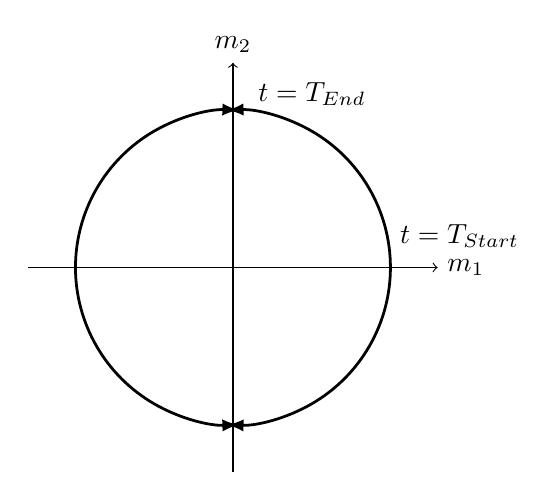
\begin{tikzpicture}[scale=2]
    % Draw the coordinate axes
    \draw[->] (-1.3,0) -- (1.3,0) node[right] {$m_1$};
    \draw[->] (0,-1.3) -- (0,1.3) node[above] {$m_2$};
    
    % Draw the circle
    % \draw (0,0) circle (1cm);

    \node[right] at (1, 0.2) {$t=T_{Start}$};
    \node[right] at (0.1, 1.1) {$t=T_{End}$};


    % Add arrows along the circle pointing to the top
    \draw[->, >=latex, line width=1pt] (0:1) arc[start angle=0,end angle=92,radius=1cm];
    \draw[->, >=latex, line width=1pt] (0:-1) arc[start angle=180,end angle=88,radius=1cm];
    \draw[->, >=latex, line width=1pt] (0:1) arc[start angle=0,end angle=-92,radius=1cm];
    \draw[->, >=latex, line width=1pt] (0:-1) arc[start angle=-180,end angle=-88,radius=1cm];
\end{tikzpicture}
\end{center}


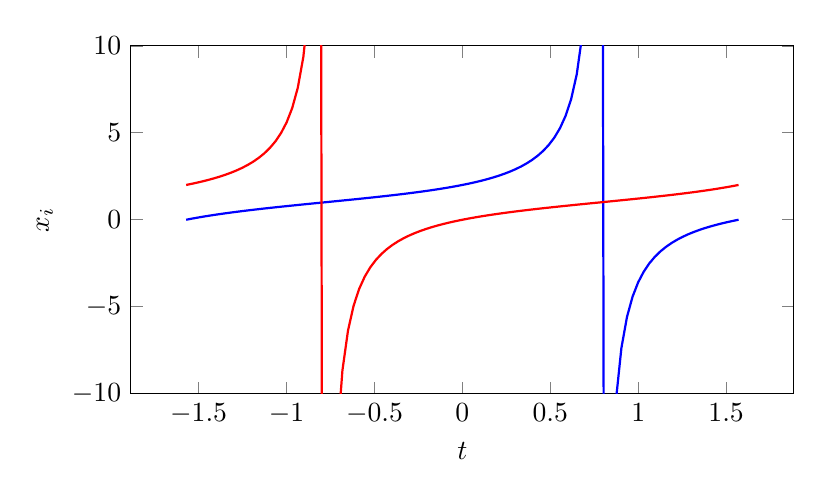
\begin{tikzpicture}
    \begin{axis}[
        xlabel={$t$},
        ylabel={$x_i$},
        domain=-pi/2:pi/2,
        samples=100,
		ymin=-10, ymax=10,
        % grid=both,
        width=10cm,
        height=6cm,
    ]
        \addplot[blue, thick] {tan(deg(x + pi/4)) + 1};
        \addplot[red, thick] {-cot(deg(x + pi/4)) + 1};
    \end{axis}
\end{tikzpicture}

\section{Numerical analysis} \label{sec:Numerical}

There are a few interesting cases to look at when $N = 2$. One could study the problem with periodic boundary conditions with a minor adjustment to the solution form
\begin{equation}
	u(x, t) = \sum_{i = 1}^{N} m_k(t) |[x - x_k(t) - L]_{2L} - L|.
\end{equation}
Where $[x]_{2L}$ is the periodic function $x \mod 2L$. This will conserve the conserved quantities and keep $\dot{u}(x,t)$ solution continuous.

At $N = 3$ there cases with collisions.


\section{Hamiltonian structure}
\todo{Todo: Add references}

\todo{Todo: Write more}

One Hamiltonian structure of the CH equation is given by the Hamiltonian
\begin{equation}
	H(x_1, \dots, x_N, m_1, \dots, m_N) = \frac{1}{2} \sum_{i,j = 1}^{N} m_i m_j e^{-|x_i - x_j|},
\end{equation}
with a canonical Poisson bracket. The Hamiltonian structure of the Hunter--Saxton equation can be derived by taking the high-frequency limit of the CH Hamiltonian structure
\begin{equation}
	H(x_1, \dots, x_N, m_1, \dots, m_N) = \frac{1}{2} \sum_{i,j = 1}^{N} m_i m_j |x_i - x_j|,
\end{equation}
with the canonical Poisson bracket.

The Hamiltonian structure of the Novikov equation is given by the same Hamiltonian as the CH equation, but with a different Poisson bracket. The Poisson bracket of the Novikov equation is given by
\begin{alignat}{3}
	\{&x_i, &x_j\} &= \sgn(x_i - x_j)(1 - e^{-2|x_i - x_j|}), \\
	\{&x_i, &m_j\} &= m_j e^{-2|x_i - x_j|}, \\
	\{&m_i, &m_j\} &= m_i m_j \sgn(x_i - x_j)e^{-2|x_i - x_j|}
\end{alignat}

A Hamiltonian structure for the high-frequency limit of the Novikov equation have not been found. One idea is to take the high-frequency limit of the Hamiltonian structure of the Novikov equation, but this does not yield the correct equations for $x_k$ and $m_k$. The Hamiltonian structure of the high-frequency limit of the Novikov equation is still an open question.

\section{Constants of motion}

\todo{Todo: Explain the algorithm further/better}\\
Two methods have been used to find constants of motion for the HF Novikov equation. One of the method will be covered in the next section. The other method is an exhaustive search algorithm. The algorithm is based on the assumption that the constants of motion are polynomials in the variables $m_k$ and $x_k$ of a fixed degree $M$ and $X$ for $m_k$ respectively $x_k$. The algorithm lists all monomials of that fixed degree
\begin{equation}
	\prod_{i=1}^{N} m_i^{a_i} x_i^{b_i},
\end{equation}
where the sum of $a_i$ is $M$ and the sum of $b_i$ is $X$. The algorithm then takes the time derivative of each monomial and forms a linear combination of them. The constants of motion are then found by finding linear combinations that are zero. The algorithm has been run both symbolically in Mathematica and numerically in C++. The algorithm has been successful up until $N = 4$, where time and numerical precision become limiting factors.

\subsection{Jacobian method}
Two or more constants of motion are said to be independent if none of them can be expressed as a function of the others. In other words, they provide unique information about the system.

To determine if a set of constants of motion are independent, the Jacobian matrix is used. Suppose there are a set of $n$ constants of motion $M_1,M_2,\dots,M_m$. These constants are functions of the variables $x_1,x_2,\dots,x_n,m_1,m_2,\dots,m_n$.

The Jacobian matrix $J$ of the functions ${M_1,M_2,\dots,M_m}$ with respect to the variables ${x_1,x_2,\dots,x_n,m_1,m_2,\dots,m_n}$ is given by:

\begin{equation}
	J = 
	\begin{pmatrix}
		\frac{\partial f_1}{\partial x_1} & \frac{\partial f_1}{\partial x_2} & \cdots & \frac{\partial f_1}{\partial x_n} & \frac{\partial f_1}{\partial m_1} & \frac{\partial f_1}{\partial m_2} & \cdots & \frac{\partial f_1}{\partial m_n} \\
		\frac{\partial f_2}{\partial x_1} & \frac{\partial f_2}{\partial x_2} & \cdots & \frac{\partial f_2}{\partial x_n} & \frac{\partial f_2}{\partial m_1} & \frac{\partial f_2}{\partial m_2} & \cdots & \frac{\partial f_2}{\partial m_n} \\
		\vdots & \vdots & \ddots & \vdots & \vdots & \vdots & \ddots & \vdots \\
		\frac{\partial f_n}{\partial x_1} & \frac{\partial f_n}{\partial x_2} & \cdots & \frac{\partial f_n}{\partial x_n} & \frac{\partial f_n}{\partial m_1} & \frac{\partial f_n}{\partial m_2} & \cdots & \frac{\partial f_n}{\partial m_n}
	\end{pmatrix}
\end{equation}

Each row of the Jacobian matrix is the gradient of one of the constants of motion. If the gradients are linearly dependent it means that one of the constants of motion can be expressed as a function of the others. Thus the rank of the Jacobian matrix is the number of independent constants of motion.

\subsection*{N = 2}

The notation for all constants of motion will be $M_{ab}$ where $a$ is the degree of $m_k$ and $b$ is the degree of $x_k$.

\begin{align}
	M_{21A} &= m_1 m_2 (x_2 - x_1), \\
	M_{20\phantom{A}} &= m_1^2\phantom{x_1} + m_2^2\phantom{x_2}, \\
	M_{21B} &= m_1^2 x_1 + m_2^2 x_2, \\
	M_{22\phantom{A}} &= m_1^2 x_1^2 + m_2^2 x_2^2. \\
\end{align}
%
The system of ODEs for $N = 2$ only has four variables so the system should have at most three functionally independent constants of motion. It can be seen that
\begin{equation}
	M_{21A}^2 = M_{20}M_{22} - M_{21B}^2.
\end{equation}

\subsection*{N = 3}

The algorithm has found the following five conserved quantities for $N = 3$.  The first two are
\begin{align}
	M_{21} &= m_1m_2(x_2 - x_1) + m_1m_3(x_3 - x_1) + m_2m_3(x_3 - x_2), \\
	M_{63} &= m_1^2m_2^2m_3^2(x_2 - x_1)(x_3 - x_1)(x_3 - x_1).
\end{align}
Let
\begin{align}
	A & = m_1^2(M_{21} + 2m_2m_3(x_3-x_2)), \\
	B & = m_2^2(M_{21} + 2m_1m_3(x_3-x_1)), \\
	C & = m_3^2(M_{21} + 2m_1m_2(x_2-x_1))
\end{align}
then the three other conserved quantities can be written as
\begin{align}
	M_{41} &= A\phantom{x_1} + B\phantom{x_2} + C\phantom{x_3} \\
	M_{42} &= Ax_1 + Bx_2 + Cx_3 \\
	M_{43} &= Ax_1^2 + Bx_2^2 + Cx_3^2
\end{align}
These conserved quantities aren't functionally independent. The Jacobian method shows that there are only four functionally independent conserved quantities. The first constant can be written as
\begin{equation}
	M_{21}^4 = M_{41}M_{43} - M_{42}^2 + 2M_{21}M_{63}.
\end{equation}

\subsection*{N = 4}

For $N = 4$ six conserved quantities have been found. The first two follow the same pattern as for $N = 3$
\begin{align}
	M_{21} = &m_1 m_2 (x_2 - x_1) + m_1 m_3 (x_3 - x_1) + m_1 m_4 (x_4 - x_1) \\ +  &m_2 m_3 (x_3 - x_2) + m_2 m_4 (x_4 - x_2) + m_3 m_4 (x_4 - x_3),\\
	M_{84} = &m_1^2m_2^2m_3^2m_4^2(x_2 - x_1)(x_3 - x_2)(x_4 - x_3)(x_4 - x_1).
\end{align}
For the next three let's define define the expression $W_i$ to be the sum of all the terms in $M_{21}$ that don't contain $m_i$. Define $A, B, C, D$ as
\begin{align}
	A &= m_1^2(M_{21} + 2W_1), \\
	B &= m_2^2(M_{21} + 2W_2), \\
	C &= m_3^2(M_{21} + 2W_3), \\
	D &= m_4^2(M_{21} + 2W_4).
\end{align}
The next  three conserved quantities can then be written as
\begin{align}
	M_{41} =& A\phantom{x_1} + B\phantom{x_2} + C\phantom{x_3} + D\phantom{x_4} \notag \\
	&+ 6m_1m_2m_3m_4 (x_1 - x_2 + x_3 - x_4) \\
	M_{42} =& Ax_1 + Bx_2 + Cx_3 + Dx_4 \notag \\
	&+ 6m_1m_2m_3m_4 (x_1x_3 - x_2x_4) \\
	M_{43} =& Ax_1^2 + Bx_2^2 + Cx_3^2 + Dx_4^2 \notag \\
	&+ 6m_1m_2m_3m_4 (x_1x_2x_3 - x_1x_2x_4 + x_1x_3x_4 - x_2x_3x_4)
\end{align}
%
Interestingly, it follows very close to the pattern of the $N = 3$ case. The only difference is that there is some extra terms that all contain $m_1m_2m_3m_4$. The last found conserved quantity is
\begin{equation}
\begin{aligned}
	M_{63} =
		 &m_1^2m_2^2m_3^2(x_2 - x_1)(x_3 - x_1)(x_3 - x_2) \\
		+&m_1^2m_2^2m_4^2(x_2 - x_1)(x_4 - x_1)(x_4 - x_2) \\
		+&m_1^2m_3^2m_4^2(x_3 - x_1)(x_4 - x_1)(x_4 - x_3) \\
		+&m_2^2m_3^2m_4^2(x_3 - x_2)(x_4 - x_2)(x_4 - x_2) \\
		+&2m_1^2m_2^2m_3m_4(x_4 - x_1)(x_2 - x_1)(x_3 - x_2) \\
		+&2m_1m_2^2m_3^2m_4(x_2 - x_1)(x_3 - x_2)(x_4 - x_3) \\
		+&2m_1m_2m_3^2m_4^2(x_3 - x_2)(x_4 - x_3)(x_4 - x_1) \\
		+&2m_1^2m_2m_3m_4^2(x_4 - x_3)(x_4 - x_1)(x_2 - x_1).
\end{aligned}
\end{equation}
Here we also find that all the conserved quantities aren't functionally independent. The Jacobian method showed that there are only five functionally independent conserved quantities, but the relation between them is still unknown.

\section{Zero curvature representation} \label{sec:ZeroCurvature}

The zero curvature representation for the Novikov equation \cite{Lundmark_2022} is
\begin{subequations}
  \label{eq:Novikov-lax}
  \begin{equation}
    \label{eq:Novikov-lax-x}
    \frac{\partial}{\partial x}
    \begin{pmatrix} \psi_1 \\ \psi_2 \\ \psi_3 \end{pmatrix} =
    \begin{pmatrix}
      0 & zm & 1 \\
      0 & 0 & zm \\
      1 & 0 & 0
    \end{pmatrix}
    \begin{pmatrix} \psi_1 \\ \psi_2 \\ \psi_3 \end{pmatrix}
    ,
  \end{equation}
  \begin{equation}
    \label{eq:Novikov-lax-t}
    \frac{\partial}{\partial t}
    \begin{pmatrix} \psi_1 \\ \psi_2 \\ \psi_3 \end{pmatrix} =
    \begin{pmatrix}
      -u u_x & \frac{u_x}{z}-u^2 mz & u_x^2 \\
      \frac{u}{z} & - \frac{1}{z^2} & - \frac{u_x}{z} - u^2 mz \\
      -u^2 & \frac{u}{z} & uu_x
    \end{pmatrix}
    \begin{pmatrix} \psi_1 \\ \psi_2 \\ \psi_3 \end{pmatrix}
    ,
  \end{equation}
\end{subequations}
%
The zero curvature condition only holds when the Novikov equation (\ref{eq:Novikov}) is satisfied. The high frequency limit of the Novikov equation is obtained by substitution $x \mapsto \epsilon x$, $t \mapsto \epsilon t$, and $m \mapsto \epsilon^{-2} m$ and letting $\epsilon \rightarrow 0$. We are left to find the correct substitution for $z$. We can do this by looking at the spatial derivative of the Lax pair and since we don't know the $x$ and $t$ factors for $\psi_1$, $\psi_2$, and $\psi_3$ we call them $A$, $B$, and $C$ respectively
\begin{equation}
\begin{pmatrix} 
	\epsilon^{-1} A \\
	\epsilon^{-1} B \\
	\epsilon^{-1} C \\
\end{pmatrix} =
\begin{pmatrix}
	0 & zm\epsilon^{-2} & 1 \\
	0 & 0 & zm\epsilon^{-2}  \\
	1 & 0 & 0
\end{pmatrix}
\begin{pmatrix} A \\ B \\ C \end{pmatrix} .
\end{equation}
Simplifying this we get
\begin{equation}
	A = z^2m^2\epsilon^{-1}A + \epsilon A,
\end{equation}
and since we don't want $A$ to go to $0$ or $\infty$ in the limit we get that $z$ should be substituted with $\epsilon^{1/2}z$.
Finally doing the substitutions $x \mapsto \epsilon x$, $t \mapsto \epsilon t$, $m \mapsto \epsilon^{-2} m$ and $z \mapsto \epsilon^{1/2}z$, and letting $\epsilon \rightarrow 0$ we get rid of the 1 in the $(1,3)$ entry in the Lax pair
\begin{equation}
\frac{\partial}{\partial x}
\begin{pmatrix} \psi_1 \\ \psi_2 \\ \psi_3 \end{pmatrix} =
\begin{pmatrix}
	0 & zm & 0 \\
	0 & 0 & zm \\
	1 & 0 & 0
\end{pmatrix}
\begin{pmatrix} \psi_1 \\ \psi_2 \\ \psi_3 \end{pmatrix}
\end{equation}
The time derivative is left unchanged. We can simplify the system even further with the following substitutions
\begin{equation}
\left\{ \begin{aligned}
	&\varphi_1 = &\psi_1, \\
	&\varphi_2 = &z\psi_2, \\
	&\varphi_3 = &z^2\psi_3.
\end{aligned} \right.
\end{equation}
By also setting $z^2 = -\lambda$ we get the following Lax pair
\begin{subequations}
\begin{equation}
\frac{\partial}{\partial x}
\begin{pmatrix} \varphi_1 \\ \varphi_2 \\ \varphi_3 \end{pmatrix} =
\begin{pmatrix}
	0 & m & 0 \\
	0 & 0 & m \\
	-\lambda & 0 & 0
\end{pmatrix}
\begin{pmatrix} \varphi_1 \\ \varphi_2 \\ \varphi_3 \end{pmatrix}
,
\end{equation}
\begin{equation}
\frac{\partial}{\partial t}
\begin{pmatrix} \varphi_1 \\ \varphi_2 \\ \varphi_3 \end{pmatrix} =
\begin{pmatrix}
	-u u_x & -\frac{u_x}{\lambda}-u^2 m & -\frac{u_x^2}{\lambda} \\
	u & \frac{1}{\lambda} & \frac{u_x}{\lambda} - u^2 m \\
	u^2\lambda & u & uu_x
\end{pmatrix}
\begin{pmatrix} \varphi_1 \\ \varphi_2 \\ \varphi_3 \end{pmatrix}
.
\end{equation}
\end{subequations}
%
%
With
\begin{equation}
	u_x = \sum_{k=1}^n m_k \sgn(x - x_k),
\end{equation}
it means that $m$ will be
\begin{equation}
	m = u_{xx} = \sum_{k=1}^n 2 m_k \delta(x - x_k),
\end{equation}
since the sign function have a jump discontinuity at $x_k$ of size 2 and the derivative of the sign function is the Dirac delta function. This means that $\varphi_1$ and $\varphi_2$ will have jump discontinuities at $x_k$ because of the Dirac delta function in their spatial derivative. $\varphi_3$ doesn't have any Dirac delta function in its spatial derivative so it will be continuous. We will assume that $x_1 < \cdots < x_n$, which will stay true at least for a time after $t = 0$ if it's true at $t = 0$. We will also use the convention that $x_0 = -\infty$ and $x_{n+1} = \infty$. Since $m = 0$ in the intervals $x_k < x < x_{k+1}$, the spatial Lax pair simplifies to $\delta_x \varphi_1 = 0$, $\delta_x \varphi_2 = 0$, and $\delta_x \varphi_3 = \varphi_1$. This means that $\varphi_1$, $\varphi_2$ and $\varphi_3$ have to be
\begin{equation}
\begin{pmatrix} \varphi_1 \\ \varphi_2 \\ \varphi_3 \end{pmatrix} =
\begin{pmatrix} A_i \\ B_i \\ -\lambda A_i x + C_i \end{pmatrix} 
\text{for } x_k < x < x_{k+1}.
\end{equation}
We can also see from the Lax pair that $\varphi_3$ is going to be continuous, while $\varphi_1$ and $\varphi_2$ is constant in the intervals with jump discontinuities at $x_k$. Let's rewrite the Lax pair in terms of $A, B, C$ instead of $\varphi_1, \varphi_2, \varphi_3$:
\begin{subequations}
  \begin{equation}
    \frac{\partial}{\partial x}
    \begin{pmatrix} A \\ B \\ C \end{pmatrix} =
    \begin{pmatrix}
      0 & m & 0 \\
      -\lambda m x & 0 & m \\
      0 & \lambda m x & 0
    \end{pmatrix}
    \begin{pmatrix} A \\ B \\ C \end{pmatrix}
	=: U(x) \begin{pmatrix} A \\ B \\ C \end{pmatrix}
    ,
  \end{equation}
  \begin{align}
    \frac{\partial}{\partial t}
    \begin{pmatrix} A \\ B \\ C \end{pmatrix} &=
    \begin{pmatrix}
      u_x X & -\frac{u_x}{\lambda} -u^2 m & -\frac{u_x^2}{\lambda} \\
      -X + \lambda u^2 m x & \frac{1}{\lambda} & \frac{u_x}{\lambda} - u^2 m \\
      \lambda X^2 & -X - \lambda u^2 m x & -u_x X
    \end{pmatrix}
    \begin{pmatrix} A \\ B \\ C \end{pmatrix} \\
	&=: V(x) \begin{pmatrix} A \\ B \\ C \end{pmatrix}
    ,
  \end{align}
\end{subequations}
where $X = u_x x - u$. This also fulfills the zero curvature condition. Call $F(x;t)$ the vector of $A, B, C$ and let $T$ be the transition matrix that takes us from $x$ to $y$ as $F(y;t) = T(y,x;t)F(x;t)$. $F$ is mostly constant with jump discontinuities at $x_k$ so we can write the jump matrix $S_k$ at $x_k$ as
\begin{equation}
\begin{aligned}
\begin{pmatrix} A_k \\ B_k \\ C_k \end{pmatrix} &= 
\begin{pmatrix}
	1 - 2\lambda m_k^2 x_k & 2m_k & 2m_k^2 \\
	-2\lambda m_k x_k & 1 & 2m_k \\
	-2\lambda^2 m_k^2 x_k^2 & 2\lambda m_k x_k & 1 + 2\lambda m_k^2 x_k
\end{pmatrix}
\begin{pmatrix} A_{k-1} \\ B_{k-1} \\ C_{k-1} \end{pmatrix} \\
&=: S_k(t) 
\begin{pmatrix} A_{k-1} \\ B_{k-1} \\ C_{k-1} \end{pmatrix}
\end{aligned}
\end{equation}
Let $T_a(t) = T(a,-a;t)$. Then at large enough $a$ we can write 
\begin{equation}
	T_a(t) = S_n(t)S_{n-1}(t) \cdots S_1(t).
\end{equation}
Since $U$ is bounded we can now write the monodromy matrix as
\begin{equation}
	M(t) = \lim_{a \rightarrow \infty} T_a(t).
\end{equation}
From corollary \ref{cor:Monodromy} we know that the time derivative of $M$ is given by $[V_0, M]$ if $V(x;t)$ goes to the same thing at $\pm \infty$. At the limits, we can know that $m$ will be zero. Our $V$ can then be split into one even and one odd part
\begin{equation}
	V(x;t) =
\begin{pmatrix}
	u_x X & 0 & -\frac{u_x^2}{\lambda} \\
	0 & \frac{1}{\lambda} & 0 \\
	\lambda X^2 & 0 & -u_x X
\end{pmatrix} +
\begin{pmatrix}
	0  & -\frac{u_x}{\lambda} & 0 \\
	-X & 0 & \frac{u_x}{\lambda} \\
	0 & -X & 0
\end{pmatrix}.
\end{equation}
So we almost have that $V(-\infty) = V(\infty)$. If
\begin{equation}
	D = 
\begin{pmatrix}
	1 & 0 & 0 \\
	0 & -1 & 0 \\
	0 & 0 & 1
\end{pmatrix},
\end{equation}
%
we can write $V(a) = DV(-a)D$. This means that 
\begin{equation}
	\partial_t T_a(t) = DV(-a;t)DT_a(t) - T_a(t)V(-a;t).
\end{equation}
Multiplying by $D$ from the left, it can be seen that the transpose of $DT_a(t)$ will be constant in time
\begin{equation}
\begin{aligned}
	\partial_t \tr(D T_a(t))
	&= \tr(D \partial_t T_a(t)) \\
	&= \tr(DDV(-a;t)DT_a(t) - DT_a(t)V(-a;t)) \\
	&= \tr(V(-a;t)DT_a(t) - DT_a(t)V(-a;t)) \\
	&= \tr([V(-a;t), DT_a(t)]) \\
	&= 0.
\end{aligned}
\end{equation}
Thus the sum $M(t;\lambda)[1,1] - M(t;\lambda)[2,2] + M(t;\lambda)[3,3]$ forms a polynomial in $\lambda$, where every coefficient is a constant of motion. It seems like this method will yield $N-1$ independent constant of motion for each $N$. Were the coefficient of the lowest and highest term of $\lambda$ respectively yield the following constants of motion
\begin{equation}
	\sum_{i=1}^{N}\sum_{j=1}^N m_i m_j |x_i - x_j|,
\end{equation}
\begin{equation}
	\prod_{i=1}^{N} m_i^2 (x_i - x_{i-1}).
\end{equation}

The transpose of $DT_a$ will be a polynomial in $\lambda$ with the following form
\begin{equation}
	C_0 + C_1 \lambda + C_2 \lambda^2 + \cdots + C_{n} \lambda^{n}.
\end{equation}

The jump matrix can be written as
\begin{equation}
	S_k = D + \hat{S_k} = D + 
	\begin{pmatrix}
		m_k \\ 1 \\ \lambda m_k x_k		
	\end{pmatrix}
	\begin{pmatrix}
		-2 \lambda m_k x_k & 2 & 2 m_k
	\end{pmatrix}.
\end{equation}
Then the $T_a$ matrix will be
\begin{equation}
	T_a = (D + \hat{S}_n)\cdots(D + \hat{S}_2)(D + \hat{S}_1).
\end{equation}
The $T_a^{(1,1)}$ and $T_a^{(3,3)}$ elements will always be a polynomial of one higher order than the $T_a^{(2,2)}$ element. $C_0$ is always independent of $x_k$ and $m_k$ and will thus not give any information about the system. $C_n$ is the coefficient of the highest order in $\lambda$. The higest order terms of the $T_a$ matrix comes from multiplying all the $\hat{S}_k$'s together
\begin{equation}
\begin{aligned}
	\hat{S}_{\text{tot}} = \hat{S}_n \cdots \hat{S}_2 \hat{S}_1 &=
	\prod_{k=1}^{n-1} L_k
	\begin{pmatrix}
		m_n \\ 1 \\ \lambda m_n x_n
	\end{pmatrix}
	\begin{pmatrix}
		-2\lambda m_1x_1 & 2 & 2 m_1
	\end{pmatrix} \\
	&= \prod_{k=1}^{n-1} L_k
	\begin{pmatrix}
		-2\lambda m_n m_1 x_1 & 2m_n & 2m_n m_1 \\
		-2\lambda m_1 x_1 & 2 & 2m_1 \\
		-2\lambda^2 m_n m_1 x_n x_1 & 2\lambda m_n x_n & 2\lambda m_n m_1 x_n
	\end{pmatrix}
\end{aligned}
\end{equation}
where $L_k$ is the dot product that comes from multiplying $S_k$ and $S_{k+1}$. So $L_k$ is
\begin{equation}
\begin{aligned}
	L_k &= 
	\begin{pmatrix}
		m_{k+1} \\ 1 \\ \lambda m_{k+1} x_{k+1}
	\end{pmatrix}
	\begin{pmatrix}
		-2\lambda m_kx_k & 2 & 2 m_k
	\end{pmatrix} \\
	&= 2\lambda m_k m_{k+1} (x_{k+1} - x_k) + 2.
\end{aligned}
\end{equation}
The $C_n$ coefficient will then be the sum of the first and third diagonal element of $S_{\text{tot}}$
\begin{equation}
	2\lambda m_n m_1 (x_n - x_1) \prod_{k=1}^{n-1} L_k
	= \prod_{i=1}^{N} m_i^2 (x_{i+1} - x_i),
\end{equation}
were in this case $x_{n+1} = x_1$.

%=========================================================================%
%
% The Appendix
%
%=========================================================================%
\newpage
\appendix

\section{Derivation of the ODE system} \label{sec:DerivationODE}

This section provides proof of that the ODE-system \eqref{eq:peakon_odes} is obtained from the PDE by plugging in the ansatz $u = \sum m_k |x - x_k|$.

\subsubsection*{Preliminaries}

The jump and the average of $f$ at $x_k$ will be defined as
\begin{equation}
	[f(x_k)] := f(x_k^+) - f(x_k^-) \quad \text{and} \quad \langle f(x_k)\rangle := \frac{f(x_k^+) + f(x_k^-)}{2},
\end{equation}
respectively. They satisfy the product rules
\begin{equation} \label{eq:dirac_product_rules}
	[fg] = \langle f\rangle[g] + [f]\langle g\rangle, \quad \quad \langle fg\rangle = \langle f\rangle\langle g\rangle + \frac{1}{4}[f][g].
\end{equation}
%
For a continuous function $f$ and a piecewise continuous function $g$ the product rule for jumps simplifies to
\begin{equation}
	[fg] = f[g].
\end{equation}
In the way the HF-Novikov equation is written here
\begin{equation}
	u_{xxt} = -u^2u_{xxx} - 3uu_xu_{xx},
\end{equation}
there is an issue with term $3uu_xu_{xx}$, since $u_x$ isn't defined at $x_k$ and $u_{xx}$ is a Dirac delta function. One way to get around that is to write the HF-Novikov equation as
\begin{equation}
	-\partial_x^2 u_t - \partial_x^2 u^2 u_x + \partial_x \frac{3}{2} u u_x^2 + \frac{1}{2}u_x^3 = 0.
\end{equation}
%
The first terms is 
\begin{equation}
	-\partial_x^2 u_t = - \sum \dot{m}_k 2 \delta_{x_k} + \sum 2 \dot{x}_k m_k \delta'_{x_k}.
\end{equation}
%
The second term $-\partial_x^2 u^2 u_x$ will have the two singular terms
\begin{equation}
	- \sum [(u^2 u_x)_x] \delta_{x_k} - \sum [u^2 u_x] \delta'_{x_k}.
\end{equation}
%
Let's first look at the $\delta'$ term at $x_k$
\begin{equation}
	- [u^2 u_x]_{x_k} = - u^2(x_k) \underbrace{[u_x(x_k)]}_{2m_k} = -2 m_k u^2(x_k).
\end{equation}
Next let's look at the $\delta$ term at $x_k$
\begin{equation}
\begin{aligned}
	- [(u^2 u_x)_x]_{x_k} &= -[2u u_x^2 + u^2 u_{xx}]_{x_k} \\
		&= - 2u(x_k) \underbrace{[u_x^2(x_k)]}_{2\langle u_x \rangle [u_x]}
		- u^2(x_k) \underbrace{[u_{xx}(x_k)]}_{=0} \\
		&= -4u(x_k) \langle u_x(x_k) \rangle \underbrace{[u_x(x_k)]}_{2m_k} = -8m_k u(x_k) u_x(x_k).
\end{aligned}
\end{equation}
The third term $\partial_x \frac{3}{2}u u_x^2$ will have one singular term
\begin{equation}
	\sum [\frac{3}{2} u u_x^2] \delta_{x_k},
\end{equation}
which at $x_k$ will be
\begin{equation}
	[\frac{3}{2}u u_x^2]_{x_k} = \frac{3}{2}u(x_k) \underbrace{[u_x^2(x_k)]}_{2\langle u_x \rangle [u_x]} = 3 \langle u_x(x_k) \rangle \underbrace{[u_x(x_k)]}_{2m_k} = 6m_k u(x_k) u_x(x_k).
\end{equation}
%
The forth term will not have any singular terms. The $\delta$ and $\delta'$ distributions are linearly independent so the terms can be split up into separate equations. At $x_k$ the sum from all the terms for $\delta$ and $\delta'$ is
\begin{equation}
\begin{aligned}
	0 = -2 \dot{m}_k - [(u^2u_x)_x]_{x_k} + [\frac{3}{2}uu_x^2]_{x_k} = -2 \dot{m}_k - 2 m_k u(x_k) u_x(x_k),
\end{aligned}
\end{equation}
respectively
\begin{equation}
\begin{aligned}
	0 = 2 \dot{x}_k m_k - [u^2u_x]_{x_k} = 2 \dot{x}_k m_k - 2m_ku^2(x_k).
\end{aligned}
\end{equation}
%
The $\dot{m}_k$ equation can be written as
\begin{equation}
	\dot{m}_k = -m_ku_x(x_k)u(x_k).
\end{equation}
It can be assumed that $m_k \neq 0$ since $\dot{m}_k = m_k \cdot (something)$ implies that either $m_k(t) = 0$ for all $t$ or $m_k(t) \neq 0$ for all $t$. If $m_k = 0$ it doesn't contribute anything to $u$ and can therefore be ignored. With $m_k \neq 0$ the expression can be divided by $m_k$ to get
\begin{equation}
	\dot{x}_k = u(x_k)^2.
\end{equation}

\section{Verification of the Lax pair for the ansatz}

Generally a function needs to be continuous for the it's multiplication with a Dirac delta function to be well defined. Which creates a problem with the multiplication of $u_x \delta_{x_k}$ since $u_x$ is not continuous at $x_k$. Therefore we will define $u_x \delta_{x_k} := \langle u_x(x_k) \rangle \delta_{x_k}$. The Lax pair formulation is
\begin{equation}
	\partial_x \Psi = \hat{U} \Psi, \qquad \partial_t \Psi = \hat{V} \Psi.
\end{equation}
In this case $\Psi = (\psi_1, \psi_2, \psi_3)^T$ and $\hat{U}$ and $\hat{V}$ are matrices. Both $\hat{U}$ and $\hat{V}$ can be split up into a regular and a singular part
%
\begin{equation}
\hat{U} = U + zmN, \qquad \hat{V} = V - zu^2mN,
\end{equation}
where
\begin{equation}
U =
	\begin{pmatrix}
	0 & 0 & 0 \\
	0 & 0 & 0 \\
	1 & 0 & 0
	\end{pmatrix},
V = 
	\begin{pmatrix}
	-u u_x & \frac{u_x}{z} & u_x^2 \\
	\frac{u}{z} & - \frac{1}{z^2} & - \frac{u_x}{z} \\
	-u^2 & \frac{u}{z} & uu_x
	\end{pmatrix},
N =
	\begin{pmatrix}
	0 & 1 & 0 \\
	0 & 0 & 1 \\
	0 & 0 & 0
	\end{pmatrix}.
\end{equation}
%
We also have that
\begin{equation}
	u = \sum m_k |x - x_k|, \quad u_x = \sum m_k \sgn(x - x_k), \quad m = u_{xx} = \sum 2 m_k \delta(x - x_k).
\end{equation}
Next we do the mixed partials
\begin{equation}
\begin{aligned}
	\partial_t \partial_x \Psi &= \partial_t (U \Psi + zmN \Psi) \\ 
	&= (\underbrace{U_t}_{=0} + UV) \Psi + (zm N \Psi)_t, \\
	\partial_x \partial_t \Psi &= \partial_t (V \Psi + zu^2mN \Psi) \\
	&= (V_x + VU) \Psi + \sum [ V \Psi ] \delta_{x_k} + (zu^2m N \Psi)_x.
\end{aligned}
\end{equation}
The mixed partials should be equal, so for simplify both parts will be put on the same side like so $\partial_t \partial_x \Psi - \partial_x \partial_t \Psi = 0$. The regular of the mixed partials is
\begin{equation}
	UV - VU - V_x =
	\begin{pmatrix}
		u u_{xx} & -\frac{u_{xx}}{z} & -2 u_x u_{xx} \\
		0 & 0 & \frac{u_{xx}}{z} \\
		0 & 0 & -u u_{xx}
	\end{pmatrix},
\end{equation}
which is identically zero, since the regular part of $u_xx$ is zero. The singular part of the mixed partials is
\begin{equation}
	(zmN \Psi)_t - \sum [V \Psi] \delta_{x_k} - (zu^2mN \Psi)_x.
\end{equation}
Using the produce rule (\ref{eq:dirac_product_rules}) we get that
\begin{equation}
	\sum [V \Psi] \delta_{x_k} = \sum \langle V \rangle [\Psi(x_k)] + [V]\langle \Psi(x_k) \rangle.
\end{equation}


%=========================================================================%
%
% Bibliography. The References are added to the file
% references.bib. Use, e.g. \cite{grote:97} to make a reference.
%
%=========================================================================%
\newpage
\bibliographystyle{plain}
\bibliography{references.bib}








\end{document}
